%% appendix.tex
%%

%% ==============================
%\chapter{Appendix}
%\label{ch:Appendix}
%% ==============================
%\renewcommand\thefigure{\thechapter.\arabic{figure}}
\appendix

%\iflanguage{english}
{\addchap{Appendix}}	% english style
%{\addchap{Anhang}}	% german style

\section{Graphs}\label{appendix:graphs}

\begin{figure}[ht]
	\centering
		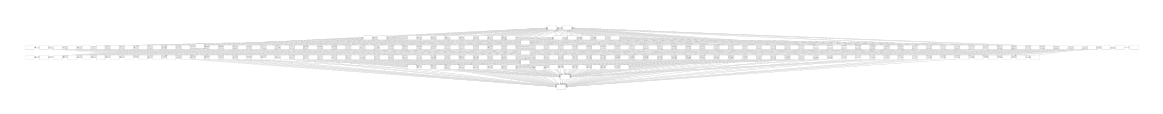
\includegraphics[width=0.90\textwidth]{figures/graphs/graphextrem.png}
	\caption{An example graph containing only $186$ nodes has over $9000$ edges.}
	\label{fig:graphextreme}
\end{figure}
\begin{figure}[ht]
	\centering
		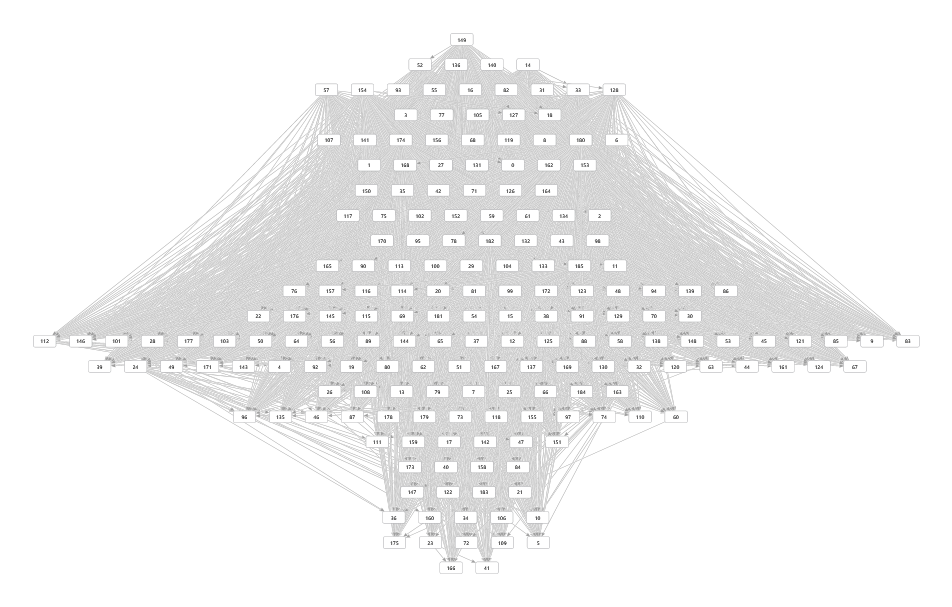
\includegraphics[width=0.90\textwidth]{figures/graphs/graphn186l22.png}
	\caption{The example graph's reduced version, which only contains unidirectional communication links. $l = 22$ can be efficiently computed in this subgraph. ($6310$ edges remain in this graph)}
	\label{fig:graphbetter}
\end{figure}
\newpage
\section{Plots}

\begin{figure}[ht]
	\centering
		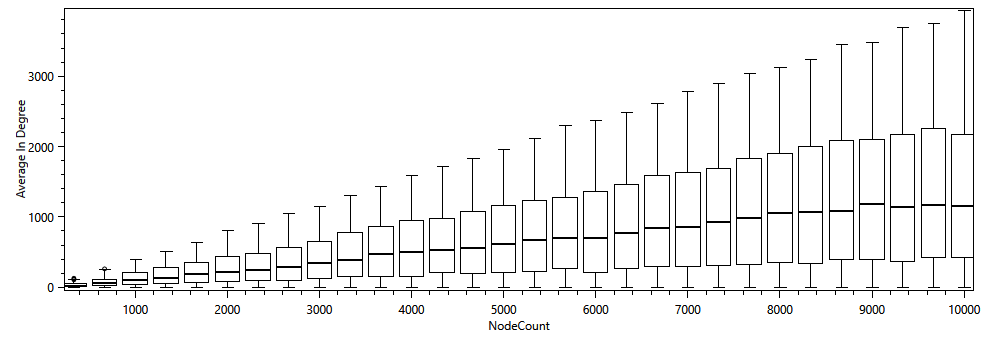
\includegraphics[width=0.90\textwidth]{figures/plots/boxplotndelta.png}
	\caption{Confirmation that $\Delta$ grows linearly with $n$ in our setting.}
	\label{fig:boxplotndelta}
\end{figure}

\begin{figure}[ht]
	\centering
		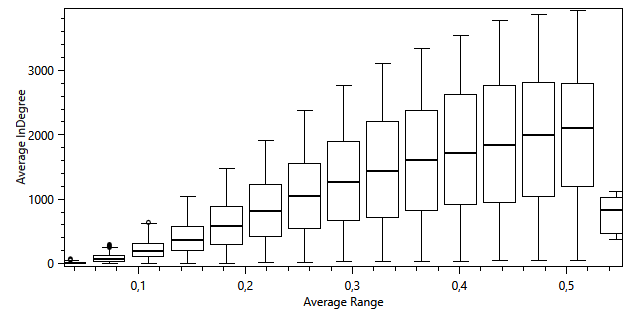
\includegraphics[width=0.90\textwidth]{figures/plots/boxplotaveragerangedelta.png}
	\caption{This plot shows that with an increase in transmission ranges, $\Delta$ increases proportionally.}
	\label{fig:boxplotaveragerangedelta}
\end{figure}



